\documentclass{article}
\usepackage{graphicx}
\usepackage{amsmath}
\usepackage[margin=1in]{geometry}
\usepackage{titling}
\usepackage{abstract}

\usepackage{tikz}
\usetikzlibrary{arrows.meta, positioning, calc, fit}
\usepackage{subcaption}

\title{Half Scramble}
\author{Lucas Gutheim}
\date{\today}

\renewcommand{\abstractnamefont}{\normalfont\bfseries}
\renewcommand{\abstracttextfont}{\normalfont}
\setlength{\absleftindent}{0pt}
\setlength{\absrightindent}{0pt}

\begin{document}
\maketitle

\begin{abstract}
We study the structure of scramble and solution paths in the Rubik's cube state space, modeled as the Cayley graph of a finitely generated group. We analyze the structural relationship between these paths and their inverses, and provide visual representations of the induced trajectories. The resulting framework emphasizes the geometric structure of solution spaces in the cube group and highlights the existence of multiple nontrivial geodesic-like paths between configurations.
\end{abstract}

\section{Introduction}

We model the Rubik's cube as the Cayley graph of a finitely generated group, where vertices correspond to cube configurations and edges correspond to generator moves.

A scramble is represented by a word $w = a_1 a_2 \cdots a_N$ acting on the identity state $e$, producing a configuration $X = w(e)$. The standard solution corresponds to the inverse word $w^{-1}$, which traces a direct reversal of the scramble path.

In this work, we instead consider the construction of an alternative solution word $v$ such that $v(X) = e$, obtained via a constrained search procedure. The constraint enforces non-backtracking behavior by disallowing immediate reversal of the last applied generator, thereby preventing trivial inversion of the scramble sequence.

This results in two distinct paths in the Cayley graph connecting $e$ and $X$: the forward scramble path induced by $w$, and an alternative solution path induced by $v$. We study the structural relationship between these paths and their inverses, and provide visual representations of the induced trajectories.

The resulting framework emphasizes the geometric structure of solution spaces in the cube group and highlights the existence of multiple nontrivial geodesic-like paths between configurations.

\newpage

\section{Setup}

Let
\[
G = \langle U, U', U^2, D, D', D^2, L, L', L^2, R, R', R^2, F, F', F^2, B, B', B^2 \rangle
\]
be the Rubik’s Cube group, where we work in the half-turn metric (HTM), so each generator counts as a single move. \\ \\
Let $e \in G$ denote the solved state.

\section{Scramble}

We begin by fixing a target length \(N\) and constructing a word
\[
w = a_1 a_2 \cdots a_N, \quad a_i \in S,
\]
where
\[
S = \{U, U', U^2, D, D', D^2, L, L', L^2, R, R', R^2, F, F', F^2, B, B', B^2\}.
\] 
This word defines a scrambled state
\[
X = w(e).
\] 

We represent the scrambling process as a path in the Cayley graph of the cube group. Figure~\ref{fig:paths1} shows the trajectory from the identity state \(e\) to a scrambled configuration \(X\), where
\[
A^i = (a_1 a_2 \cdots a_i)(e), \quad 1 \le i \le N.
\]

\vspace{.5cm}

\begin{figure}[h]
\begin{center}
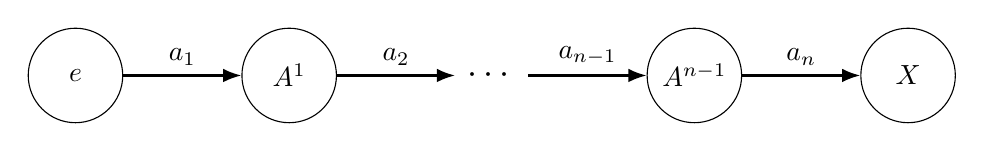
\begin{tikzpicture}[
    node distance=1.5cm,
    state/.style={draw, circle, minimum size=1.2cm},
    arrow/.style={-Latex, thick}
]

% endpoints and a few key intermediates
\node[state] (A0) {$e$};
\node[state, right=of A0] (A1) {$A^1$};

\node[right=of A1, scale=1.3] (dots) {$\cdots$};

\node[state, right=of dots] (An1) {$A^{n-1}$};
\node[state, right=of An1] (An) {$X$};

% arrows
\draw[arrow] (A0) -- node[midway, above] {$a_1$} (A1);
\draw[arrow] (A1) -- node[midway, above] {$a_2$} (dots);

\draw[arrow] (dots) -- node[midway, above] {$a_{n-1}$} (An1);
\draw[arrow] (An1) -- node[midway, above] {$a_n$} (An);

\end{tikzpicture}

\caption{
Trajectory in the Cayley graph of the cube group corresponding to the scramble word $(a_1 a_2 \cdots a_N)$ applied to the identity state $e$, yielding intermediate states $A^i$ and final state $X$.
}
\label{fig:paths1}
\end{center}
\end{figure}



\section{Solve}
Next, we compute an alternative solution from \(X\) back to \(e\) using a modified IDA* search. This produces a word
\[
v = b_1 b_2 \cdots b_k, \quad b_i \in S,
\]
such that
\[
v(X) = e.
\]

To prevent the search from immediately undoing the scramble, we impose a constraint on the first move:
\[
b_1 \neq a_n^{-1}.
\]
This blocks the trivial reversal of the final step of \(w\), forcing the search to explore alternative geodesics in the Cayley graph.

Thus, we obtain two distinct words relating \(e\) and \(X\):
\[
X = w(e), \quad e = v(X),
\]
with \(v \neq w^{-1}\) due to the imposed constraint.

Figure~\ref{fig:paths2} shows the trajectory from the identity state \(e\) to a scrambled configuration \(X\) via the word \(w\), as well as the reverse trajectory from \(X\) to \(e\) via the word \(v\).

The intermediate states along the solution path are defined by
\[
B^i = (b_1 b_2 \cdots b_i)(e), \quad 1 \le i \le k.
\]

During the search procedure, we forbid immediate backtracking by disallowing a generator that would undo the last move of the scramble; this restriction is highlighted in red in the figure.


\vspace{1cm}
% =======================
% (B) MULTIPLE SOLUTIONS
% =======================
\begin{figure}[h]
\begin{center}
    
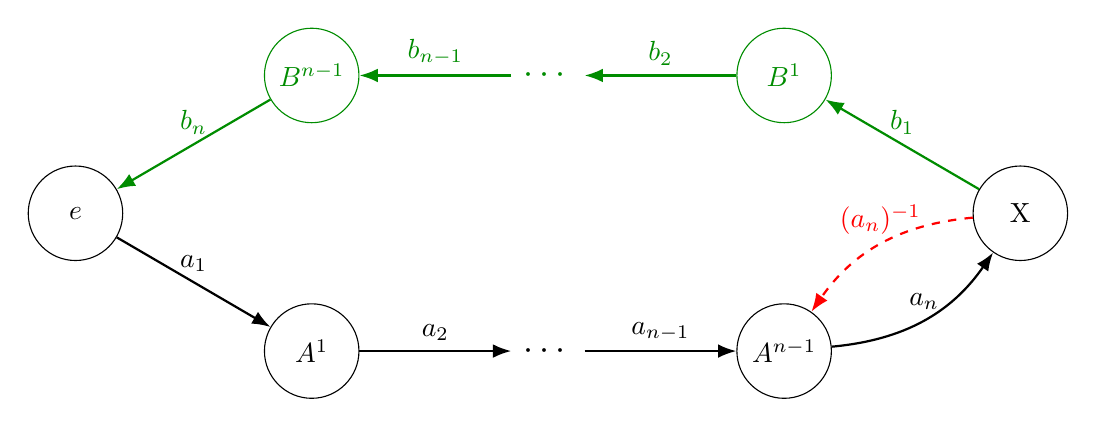
\begin{tikzpicture}[
    state/.style={draw, circle, minimum size=1.2cm},
    state_sol/.style={draw, circle, minimum size=1.2cm, green!55!black},
    arrow/.style={-Latex, thick},
    blocked/.style={-Latex, thick, dashed, red},
    arrow_sol/.style={-Latex, thick, green!55!black},
]

\node[state] (e) at (0,0) {$e$};
\node[state] (a1) at (3,-1.75) {$A^1$};
\node[scale=1.3] (adots) at (6, -1.75) {$\cdots$};
%\node[state] (s2) at (6,0) {$A^2$};
\node[state] (a3) at (9,-1.75) {$A^{n-1}$};
\node[state] (scr) at (12,0) {X};

\node[state_sol] (b1) at (9,1.75) {$B^1$};
\node[scale=1.3, green!55!black] (bdots) at (6,1.75) {$\cdots$};
\node[state_sol] (b3) at (3,1.75) {$B^{n-1}$};


% edges top
\draw[arrow] (e) -- node[midway, above] {$a_1$} (a1);
\draw[arrow] (a1) -- node[midway, above] {$a_2$} (adots);
\draw[arrow] (adots) -- node[midway, above] {$a_{n-1}$} (a3);
\draw[arrow] (a3) to[bend right=25] node[midway, above] {$a_n$}  (scr);
\draw[blocked] (scr) to[bend right=25] node[midway, above] {$(a_n)^{-1}$} (a3);


% edges bottom
\draw[arrow_sol] (scr) -- node[midway, above] {$b_1$} (b1);
\draw[arrow_sol] (b1) -- node[midway, above] {$b_2$} (bdots);
\draw[arrow_sol] (bdots) -- node[midway, above] {$b_{n-1}$} (b3);
\draw[arrow_sol] (b3) -- node[midway, above] {$b_n$} (e);

\end{tikzpicture}

\caption{Trajectories in the Cayley graph induced by the scramble word $w$ and the alternative solution word $v$. The forward path maps $e \to X$, while the reverse path maps $X \to e$. Red edges indicate forbidden backtracking moves during the search, preventing immediate cancellation of the scramble.}
\label{fig:paths2}
\end{center}
\end{figure}

\section{Reversal}

For any word
\[
M = m_1 m_2 \cdots m_n,
\]
its inverse is defined as
\[
M^{-1} = m_n^{-1} \cdots m_2^{-1} m_1^{-1}.
\]
Applying this to \(w\) and \(v\), we have:
\[
w^{-1}(X) = e, \quad v^{-1}(e) = X.
\]
Figure~\ref{fig:paths3} shows the inverse trajectories corresponding to $w$ and $v$.

\vspace{.5cm}
\begin{figure}[h]
\begin{center}
    
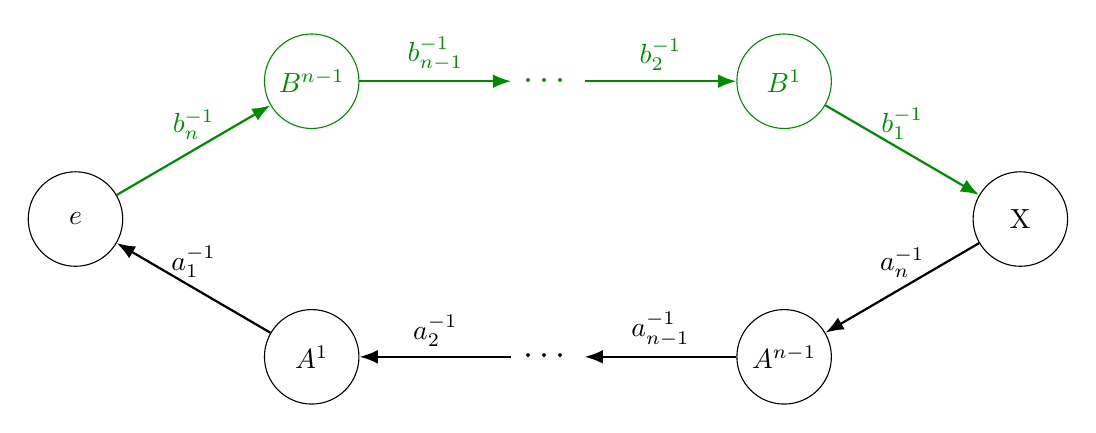
\begin{tikzpicture}[
    state/.style={draw, circle, minimum size=1.2cm},
    state_sol/.style={draw, circle, minimum size=1.2cm, green!55!black},
    arrow/.style={-Latex, thick},
    arrow_sol/.style={-Latex, thick, green!55!black}
]

\node[state] (e) at (0,0) {$e$};
\node[state] (a1) at (3,-1.75) {$A^1$};
\node[scale=1.3] (adots) at (6, -1.75) {$\cdots$};
%\node[state] (s2) at (6,0) {$A^2$};
\node[state] (a3) at (9,-1.75) {$A^{n-1}$};
\node[state] (scr) at (12,0) {X};

\node[state_sol] (b1) at (9,1.75) {$B^1$};
\node[scale=1.3, green!55!black] (bdots) at (6,1.75) {$\cdots$};
\node[state_sol] (b3) at (3,1.75) {$B^{n-1}$};


% edges top
\draw[arrow] (a1) -- node[midway, above] {$a_1^{-1}$} (e);
\draw[arrow] (adots) -- node[midway, above] {$a_2^{-1}$} (a1);
\draw[arrow] (a3) -- node[midway, above] {$a_{n-1}^{-1}$} (adots);
\draw[arrow] (scr) -- node[midway, above] {$a_n^{-1}$}  (a3);

% edges bottom
\draw[arrow_sol] (b1) -- node[midway, above] {$b_1^{-1}$} (scr);
\draw[arrow_sol] (bdots) -- node[midway, above] {$b_2^{-1}$} (b1);
\draw[arrow_sol] (b3) -- node[midway, above] {$b_{n-1}^{-1}$} (bdots);
\draw[arrow_sol] (e) -- node[midway, above] {$b_n^{-1}$} (b3);

\end{tikzpicture}

\caption{Cayley graph representation of the scramble and solution structure. The diagram shows the traversals of the reverse paths $w^{-1}$ which maps $X \to e$ and $v^{-1}$ which maps $e \to X$.}
\label{fig:paths3}
\end{center}
\end{figure}

\newpage

\section{Conclusion}

We have analyzed the structure of scramble and solution paths in the Cayley graph of the
Rubik's Cube group, demonstrating that the non-backtracking constraint $b_1 \neq a_n^{-1}$
forces the IDA* search to produce an alternative geodesic-like path $v \neq w^{-1}$
between the identity $e$ and the scrambled configuration $X$.

The two resulting word pairs $(w, v^{-1})$ and $(w^{-1}, v)$ define a natural puzzle
structure: given $v^{-1}$ as a sequence of moves to apply to a solved cube, the solver
is tasked with recovering $w^{-1}$, the unique length-$N$ reversal of the original
scramble. This construction guarantees that a solution of the prescribed length always
exists, while the non-backtracking constraint ensures that $v^{-1}$ provides no
immediately obvious path to it.

More broadly, this framework illustrates that the local geometry of the Cayley graph
admits multiple nontrivial paths between any two configurations, and that constrained
search procedures can systematically exploit this structure. Future directions include
analyzing the distribution of path lengths $k = |v|$ relative to $N = |w|$, and
characterizing the degree to which alternative geodesics diverge from the canonical
inverse path in the half-turn metric.

\end{document}
